\chapter{Traitement du son}  

Le traitement du son a pour objectif d'améliorer la qualité de signaux au format audio, de les compresser ou encore d'en extraire une information. On distingue généralement les signaux analogiques représentés par des flux continus de données des signaux digitaux représentés par une séquence de symboles binaires.

{\footnotesize
\begin{itemize}
\item Logiciel\footnote{Le logiciel \emph{Audacity} est librement téléchargeable : \url{http://www.audacityteam.org/}} : \emph{Audacity 2.0} 
\item Prérequis : aucun
\item Matières concernées : anglais.
\item Compétences : 
        \begin{itemize}
        \item passer une piste stéréo en mono ;
        \item ajouter une piste ;
        \item copier et coller une partie de piste ;
        \item déplacer une partie de piste (glissement temporel)
        \item rendre silencieuse une partie d'une piste ;
        \item supprimer et raccorder ;
        \item réaliser un fondu en ouverture ou en fermeture ;
        \item exporter un projet au format MP3 ou WAV.
        \end{itemize}
\item Cette fiche est à réaliser :
        \begin{itemize}
        \item avant les vacances de printemps en anglais (séance 1) ;
        %\item avant la fin du semestre de cours en musique (séance 2). 
        \end{itemize}
\end{itemize}
}% fin du footnotesize




\emph{Audacity} est un enregistreur et éditeur audio libre et facile d'utilisation. Il permet d'enregistrer du son (enregistrement multi-pistes), puis d'effectuer un montage : copier, coller, couper, ajouter des effets sonores, etc. Il permet également de convertir les fichiers sons dans une grande variété de formats : MP3, WAV, OGG, etc. 














%
%
%  S  É  A  N  C  E     I
%
%

%\newpage
%\phantom{rien}
\newpage

\section{Séance 1 : composer une phrase en anglais}\label{ficheSon5e1}


\subsection{Premiers pas avec Audacity}\index{Audacity!Interface graphique}\index{Interface graphique (Audacity)}\label{Son1Interface}

La figure ci-dessous montre un projet multi-pistes en cours d'élaboration à l'aide du logiciel \emph{Audacity}. Lorsqu'on appuie sur le bouton \texttt{Lecture} 
\includegraphics[width=.4cm]{./images/son01/boutonPlay}, toutes les pistes sont lues en même temps. Ceci permet par exemple de réaliser un montage avec de la voix, de la musique en arrière plan et des bruitages.

\uneimageici{./images/son01/audacityMultipiste}{.8\textwidth}

Nous allons détailler quelque peu l'interface graphique.\\

\begin{itemize}
\item \textbf{La barre de menu principale}\index{Audacity!Barre de menu principale}\index{Barre de menu principale (Audacity)}\label{Son1BarreMenu}

\begin{minipage}[c]{.48\textwidth}
\centering%
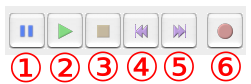
\includegraphics[angle=0,width=.5\textwidth]{./images/son01/barre_1nb}
\end{minipage}\hfill%
\begin{minipage}[c]{.48\textwidth}
\begin{tabular}{lll}
\circled{1} Pause  & & \circled{4} Saut au début \\
\circled{2} Lecture & &\circled{5} Saut à la fin  \\
\circled{3} Stop  & &\circled{6} Enregistrement\\
\end{tabular}
\end{minipage}

\vspace{12pt}\item \textbf{La palette d'outils à disposition}\index{Audacity!Palette d'outils}\index{Palette d'outils (Audacity)}\label{Son1Outils}

\begin{minipage}[c]{.17\textwidth}
\centering%
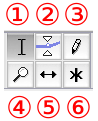
\includegraphics[angle=0,width=.7\textwidth]{./images/son01/barre_2nb}
\end{minipage}\hfill%
\begin{minipage}[c]{.78\textwidth}
\begin{tabular}{p{6cm}lp{6cm}}
\circled{1} Outil de sélection : permet de sélectionner une région && \circled{4} Outil de zoom \\
\circled{2} Outil de niveau (enveloppe) : permet de changer le volume localement && \circled{5} Outil de glissement temporel : permet de déplacer dans le temps l'enregistrement \\
\circled{3} Outil de dessin d'onde : permet de modifier la forme de l'onde && \circled{6} Mode multi-outils \\
\end{tabular}
\end{minipage}

\vspace{12pt}\item \textbf{Réglage des volumes d'entrée/sortie}\index{Audacity!Réglage des volumes}\index{Réglage des volumes (Audacity)}\label{Son1VolumesES}

Les vu-mètres de sortie 
\includegraphics[angle=0,width=.6cm]{./images/son01/hp} et d'entrée 
\includegraphics[angle=0,width=.6cm]{./images/son01/micro} (figure à gauche ci-dessous) permettent de visualiser le volume de sortie ou d'enregistrement. Si ceux-ci ne sont pas satisfaisants (trop faibles ou saturation), alors il est possible de les ajuster grâce aux deux glissières voisines (figure à droite ci-dessous).

\deuximagesici{./images/son01/barre_3}{.8\textwidth}{./images/son01/barre_4}{.8\textwidth}    


La glissière accompagnant la flèche verte (
\includegraphics[angle=0,width=.4cm]{./images/son01/fleche_verte}) permet de modifier la vitesse de lecture.

\end{itemize}



\subsection{Pour bien démarrer...}

Dès que vous avez ouvert un nouveau fichier dans \emph{Audacity}, sauvegardez-le au format Nom-seance1.mp3: dans le menu \texttt{Fichier}, choisir \texttt{Enregistrer}. Pendant que vous travaillez, pensez à sauvegarder régulièrement votre travail (raccourci clavier \texttt{Cmd + s}).   

\uneimageici{./images/generales/clavierCmdS}{.4\textwidth}


\subsection{Sujet de l'activité...}

\boiteEnonceLarge{%
Le but de cette séance est de composer une phrase en anglais à l'aide de mots enregistrés, d'y ajouter quelques effets sonores et/ou une bande son, puis d'exporter le résultat au format MP3. La liste de mots qu'il est possible d'utiliser est donnée ci-dessous.

{\footnotesize 
\begin{center}
\begin{tabular}{|c|c|c|c|c|c|c|c|}
\hline
\multirow{2}{*}{nouns} & \multirow{2}{*}{adjectives} & \multirow{2}{*}{adverbs} & \multirow{2}{*}{verbs} & personal & \multirow{2}{*}{articles} & prepo- & possessive \\
 &  &  &  & pronouns &  & sitions & pronouns \\ \hline

witch&big&always&fall&I&a &up&my\\ \hline
cat&yellow&yesterday&save&you&the &in&your\\ \hline
superheroe&funny&silently&fly&he&&out&his\\ \hline
yogurt&disgusting&kindly&shine&she &&of&her\\ \hline
moon&black&again&appear&it&&off&their\\ \hline
teacher&stinky&inside&jumped&we&&on&its\\ \hline
book&small&entirely&will eat&they&&at&\\ \hline
mum&nasty&often&hide&me&&to&\\ \hline
tree&huge&never&killed&&&over&\\ \hline
bacon&tasty&now&walk&&&&\\ \cline{2-8} 
sandwich&&cheerfully&drive&&&&\\ \hline
&&tomorrow&write&&&&\\ \hline
&&&tell a secret&&&&\\ \hline
&&&ate&&&&\\ \hline
&&&appeared&&&&\\ \hline
&&&hides&&&&\\ \hline
&&&will shine&&&&\\ \hline
\end{tabular}
\end{center}
}% fin footnotesize
}

\boiteEnonceLarge{
Pour parvenir à ce résultat, vous devrez effectuer les étapes suivantes :
%\vspace{12pt}

\begin{enumerate}
\item Composer une phrase en utilisant les mots ci-dessus.

\vspace{6pt}

\dotfill 

\vspace{6pt}

\dotfill 

\vspace{6pt}

\dotfill 

\vspace{6pt}

\dotfill 

\vspace{6pt}



\item Ouvrir dans \emph{Audacity} le fichier son qui contient tous les mots (il est disponible sur la page Teams de votre cours). Les mots sont enregistrés dans l'ordre du tableau ci-dessus, colonne par colonne.
\item Enregistrer votre projet sur le \texttt{Bureau} de l'ordinateur (menu \texttt{Fichier} puis \texttt{Enregistrer}). Penser à sauvegarder régulièrement pendant que vous travaillez (\texttt{Cmd + s}).   
\item Ajouter plusieurs nouvelles pistes mono (une par mot de votre phrase). 
\setcounter{tmp}{\value{enumi}}  
\end{enumerate}
\begin{enumerate}
\setcounter{enumi}{\value{tmp}}
\item Chercher dans le fichier son fourni chacun des mots dont vous avez besoin pour créer votre phrase et en effectuant des copier-coller, coller-les chacun dans une nouvelle piste.
\item Ajuster si nécessaire le volume de chaque piste.
\item Une fois la phrase composée, se rendre sur le site \url{http://soundbible.com} pour y télécharger des effets sonores. Ce site est une bibliothèque d'effets sonores sous \emph{licence libre} qu'il est donc possible d'utiliser et de modifier librement\footnote{Pour obtenir davantage d'informations sur les licences libres, se rendre sur le site de \emph{Creative Commons} \url{https://creativecommons.fr/}.}.
        \begin{enumerate}
        \item Utiliser le champ de recherche situé en haut à droite du site (recherche à effectuer en langue anglaise).
        \item Lorsque vous avez trouvé un effet sonore qui vous convient, cliquer sur son nom, puis le télécharger au format WAV. Choisir comme emplacement le \texttt{Bureau} de l'ordinateur afin de le retrouver facilement.
        \item L'ouvrir alors dans \emph{Audacity}, puis en effectuant un copier-coller, l'ajouter sur une nouvelle piste de votre projet. Remarque : si le son est au format stéréo, il faudra préalablement le convertir en mono (voir pour cela la section \vref{Son1stereoMono}). 
        \end{enumerate}
\item Ajouter si nécessaire des fondus en ouverture ou fermeture afin d'améliorer le rendu sonore de votre composition.
\item Une fois votre travail terminé, exporter le projet au format MP3 (le fichier doit être nommé à partir de votre nom : \texttt{Nom-seance1.mp3}) et le rendre sur la plateforme Teams à l'endroit indiqué par votre enseignant (si nécessaire, se reporter à la fiche méthode \emph{Remettre son devoir}, page \pageref{TeamsRemettreDevoir}). 
\end{enumerate}

}% fin énoncé

\textbf{Pour obtenir de l'aide, rendez-vous à la page \pageref{Son5eOutils}}

\vfill

%\cadre{Pensez à sauver régulièrement votre travail en appuyant sur \texttt{Cmd + S} ou à partir du menu \texttt{Fichier} en choisissant \texttt{Enregistrer}.

%\uneimageici{./images/generales/clavierCmdS}{.5\textwidth}
%}

\subsection{Pour aller plus loin...}

\vfill

\phantom{rien} 

\newpage

% AIDE 

\section{Aide pour réaliser l'activité}\label{Son5eOutils}

Les outils dont vous aurez besoin pour cette séance sur le traitement du son sont décrits ci-dessous :

\begin{itemize}   
\item passer une piste stéréo en mono, voir section \vref{Son1stereoMono} ;
\item ajouter une piste, voir section \vref{Son1ajouterPiste} ;
\item copier et coller une partie de piste, voir section \vref{Son1copierColler} ;
\item déplacer une partie de piste (glissement temporel), voir section \vref{Son1glissement}
\item rendre silencieuse une partie de piste, voir section \vref{Son1silence} ;
\item supprimer et raccorder, voir section \vref{Son1couperRaccorder} ;
\item réaliser un fondu en ouverture ou en fermeture, voir section \vref{Son1fondu}.
\item exporter un projet au format MP3 ou WAV, voir section \vref{Son1export}.
\end{itemize} 



\subsection{Passer une piste stéréo en mono}\index{Audacity!Stéréo vers mono}\index{Stéréo vers mono (Audacity)}\label{Son1stereoMono} 

Lorsqu'on ouvre un fichier son dans le logiciel \emph{Audacity}, il est souvent en \emph{stéréo}, c'est-à-dire que la piste contenant le son est coupée en deux canaux : un canal gauche, et un canal droit (chaque canal étant joué par une enceinte différente). Pour simplifier la prise en main du logiciel, nous allons travailler en \emph{mono} (la même bande son est jouée par toutes les enceintes). Il est donc parfois nécessaire de transformer une piste stéréo en mono, ce qui est possible en se rendant dans le menu \texttt{Pistes} et en choisissant \texttt{Piste stéréo vers mono}.    

\uneimageici{./images/son01/audacityStereoMono1}{.9\textwidth} 

Le résultat obtenu est montré ci-dessous : les informations des deux canaux de la piste stéréo sont fusionnées dans une piste mono.

\uneimageici{./images/son01/audacityStereoMono2}{.9\textwidth}




\subsection{Ajouter une piste}\index{Audacity!Ajouter une piste}\index{Ajouter une piste (Audacity)}\label{Son1ajouterPiste}

Pour effectuer un montage son, il faut ajouter au projet en cours de réalisation de nouvelles pistes vides. Pour cela, il faut se rendre dans le menu \texttt{Pistes} puis choisir \texttt{Ajouter nouvelle...} puis \texttt{Piste mono}.   

\uneimageici{./images/son01/audacityAjouterPiste1}{.9\textwidth}

La figure ci-dessous montre la nouvelle piste vide qui a été ajoutée au projet.

\uneimageici{./images/son01/audacityAjouterPiste2}{.9\textwidth}





\subsection{Copier et coller une partie de piste}\index{Audacity!Copier et coller}\index{Copier et coller (Audacity)}\label{Son1copierColler} 

En utilisant l'\emph{outil de sélection} 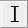
\includegraphics[width=.5cm]{./images/son01/audacityIconeSelection} (figure à gauche ci-dessous), sélectionner la partie de la piste qui doit être copiée (figure à droite ci-dessous).

\deuximagesPGici{./images/son01/audacityOutilSelection}{.8\textwidth}
                {./images/son01/audacitySelection1}{\textwidth}


Dans le menu \texttt{Édition}, choisir \texttt{Copier}. Il est également possible d'utiliser le raccourci clavier \texttt{Cmd + C}.   

\uneimageici{./images/son01/audacitySelection2}{.9\textwidth}

Sur une nouvelle piste, cliquer à l'endroit où la sélection doit être collée : une barre apparaît à l'endroit où le collage va avoir lieu (\textbf{la barre coïncide avec le début de la partie qui sera collée}). Dans le menu \texttt{Édition}, choisir ensuite \texttt{Coller}. Il est également possible d'utiliser le raccourci clavier \texttt{Cmd + V}.  

\uneimageici{./images/son01/audacitySelection3}{.9\textwidth}

Le résultat obtenu est montré ci-dessous. Il est ensuite possible de repositionner le morceau collé à l'aide de l'outil de glissement temporel 
\includegraphics[width=.5cm]{./images/son01/audacityIconeGlissement} (se reporter à la section \vref{Son1glissement}). 

\uneimageici{./images/son01/audacitySelection4}{.6\textwidth}


\subsection{Déplacer une partie de piste (glissement temporel)}\index{Audacity!Outils de glissement temporel}\index{Glissement temporel (Audacity)}\label{Son1glissement} 

En utilisant l'outil de \emph{glissement temporel} 
\includegraphics[width=.5cm]{./images/son01/audacityIconeGlissement}, (figure à gauche ci-dessous), il est possible de déplacer des parties sur une piste. Il suffit pour cela de cliquer à l'aide de la souris sur la partie à déplacer (figure à droite ci-dessous, remarquer le curseur en forme de double flèche), puis de la positionner à l'endroit souhaité.

\deuximagesPGici{./images/son01/audacityGlissement3}{.7\textwidth}%
                {./images/son01/audacityGlissement2}{.9\textwidth}




\subsection{Rendre silencieuse une partie de piste}\index{Audacity!Rendre silencieux}\index{Silence (Audacity)}\label{Son1silence}

\emph{Rendre silencieux} une partie de piste signifie diminuer le volume du son jusqu'à ce qu'on n'entende plus rien.

Pour rendre silencieuse une partie de piste, il suffit de la sélectionner en utilisant l'outil de sélection 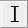
\includegraphics[width=.5cm]{./images/son01/audacityIconeSelection} puis choisir dans le menu \texttt{Édition}, \texttt{Supprimer l'audio} puis \texttt{Silence Audio}. Il est également possible de cliquer directement sur l'icône silence audio 
\includegraphics[width=.5cm]{./images/son01/audacityIconeSilence}.

\uneimageici{./images/son01/audacitySilence1}{.9\textwidth}

La zone sélectionnée apparaît alors plate : il n'y a plus de son.

\uneimageici{./images/son01/audacitySilence2}{.9\textwidth}




\subsection{Supprimer et raccorder}\index{Audacity!Raccorder}\index{Raccorder (Audacity)}\label{Son1couperRaccorder} 

\emph{Raccorder} signifie supprimer une partie de la piste mais sans créer de silence : la partie se trouvant \emph{avant} la zone supprimée se retrouve alors collée à la partie située \emph{après}.

Pour couper et raccorder une partie de la piste, il faut tout d'abord la sélectionner en utilisant l'outil de sélection 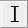
\includegraphics[width=.5cm]{./images/son01/audacityIconeSelection} puis de choisir dans le menu \texttt{Édition}, \texttt{Supprimer l'audio} puis \texttt{Supprimer et raccorder}. Il est également possible de cliquer directement l'icône raccorder 
\includegraphics[width=.5cm]{./images/son01/audacityIconeRaccorder}.

\uneimageici{./images/son01/audacityRaccorder1}{.9\textwidth}

La figure ci-dessous montre que la partie sélectionnée a disparu (elle était située à l'endroit où se trouve le curseur).

\uneimageici{./images/son01/audacityRaccorder2}{.9\textwidth}





\subsection{Réaliser un fondu en ouverture ou en fermeture}\index{Audacity!Fondu}\index{Fondu (Audacity)}\label{Son1fondu}

Réaliser un \emph{fondu en ouverture} signifie augmenter petit à petit le volume de la piste jusqu'au volume désiré. Ceci permet par exemple de faire démarrer un fond musical sans choquer l'oreille de l'auditeur.

Pour réaliser un fondu en ouverture, il faut tout d'abord sélectionner la zone à l'aide de l'outil de sélection  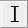
\includegraphics[width=.5cm]{./images/son01/audacityIconeSelection} puis dans le menu \texttt{Effets}, choisir \texttt{Fondre en ouverture}.  

\uneimageici{./images/son01/audacityFonduOuverture1}{.9\textwidth}

Le résultat obtenu est montré sur la figure ci-dessous : on voit clairement le volume du son qui augmente petit à petit dans la zone sélectionnée.

\uneimageici{./images/son01/audacityFonduOuverture2}{.9\textwidth}

De la même façon il est possible d'effectuer un \emph{fondu en fermeture} : le volume de la zone sélectionnée diminue alors petit à petit jusqu'au silence. 


\subsection{Modifier le volume d'une piste}\index{Audacity!Modifier le volume}\index{Volume, modifier (Audacity)}\label{Son1volume}

Pour modifier le volume d'une piste, il faut utiliser le curseur situé au début de chaque piste, comme montré sur la figure ci-dessous.

\uneimageici{./images/son01/audacityVolume}{.15\textwidth}

On peut également rendre complètement muet la piste en cliquant sur le bouton \texttt{Muet}. 



\subsection{Exporter un projet au format MP3 ou WAV}\index{Audacity!Exporter en MP3 ou WAV}\index{MP3 export (Audacity)}\index{WAV export (Audacity)}\label{Son1export} 

Pour exporter un projet au format MP3 (format compressé avec pertes) ou WAV (format non compressé), il faut se rendre dans le menu \texttt{Fichier} puis choisir \texttt{Exporter...}

\vspace{6pt}

Dans la boîte de dialogue qui s'ouvre alors, choisir le nom du fichier (\circled{1} sur la figure ci-dessous), l'emplacement où le fichier doit être enregistré \circled{2} (ici le \texttt{Bureau}), le format du fichier \circled{3} (ici le projet sera exporté au format MP3, mais il est également possible de choisir le format WAV), puis cliquer sur le bouton \texttt{OK} \circled{4}.       

\uneimageici{./images/son01/audacityExporter}{\textwidth}

Pour les boîtes de dialogues suivantes, conserver les options par défaut et cliquer sur le bouton \texttt{OK} pour réaliser l'export. 

%\subsection{}\index{Audacity!}\index{ (Audacity)}\label{Son1} 
%\uneimageici{./images/son01/}{.5\textwidth}


